\documentclass[fleqn, 11pt]{article}

%% =============================== PACKAGES ================================= %%
\usepackage[margin=0.8in]{geometry}
\usepackage[english]{babel}
\usepackage{amsmath, amsfonts, amsthm, amssymb}
\usepackage[dvipsnames]{xcolor}
\usepackage{graphicx, tikz}
\usepackage{caption, subcaption}
\usetikzlibrary{arrows.meta}
\usetikzlibrary{decorations.pathreplacing,angles,quotes}
\usetikzlibrary{shapes}
% \usepackage{wrapfig}
\usepackage{bm}
\usepackage{cases}
\usepackage{hyperref}
\usepackage{verbatim}
\usepackage{nicefrac}
% \usepackage{mathtools}
% \usepackage{algpseudocode}
% \usepackage[chapter]{algorithm}
% \usepackage{cool}
% \usepackage{multirow}

% \setlength {\marginparwidth }{2cm}
% \usepackage{todonotes}

% \usepackage[outline]{contour} % To add contour around text

% \usepackage{kpfonts}
\usepackage{fourier}
% \usepackage{txfonts} % Times New Roman
% \usepackage{ebgaramond} % Garamond

% \usepackage[nouppercase, signatures]{frontespizio}

% \usepackage{showframe} % to show page margins

%% ============================ ENVIRONMENTS ================================ %%
% Algorithm
% \renewcommand{\algorithmicrequire}{\textbf{Input:}}
% \renewcommand{\algorithmicensure}{\textbf{Output:}}
% \algnewcommand{\LeftComment}[1]{\Statex \(\triangleright\) #1}

% Theorems
\theoremstyle{definition}
\newtheorem{mydef}{Definition}[section]
\theoremstyle{plain}
\newtheorem{thm}{Theorem}[section]
\newtheorem{prop}{Proposition}[section]
\newtheorem{cor}{Corollary}[section]
\newtheorem{lmm}{Lemma}[section]
\newtheorem{pbm}{Problem formulation}[section]
\theoremstyle{remark}
\newtheorem{rmk}{Remark}[section]
\newtheorem{xmpl}{Example}[section]

\linespread{1.0} % interlinea
% \contourlength{2.3pt} % spessore contorno per testo contornato

% \usepackage{natbib}
% \usepackage{bibentry}

\title{Dynamic Movement Primitives}
\author{Michele Ginesi, Ph.D. \\ \href{https://sites.google.com/view/michele-ginesi}{https://sites.google.com/view/michele-ginesi}}
\date{Modeling Week 2022 - University of Verona}

\begin{document}
\maketitle
\begin{center}
    These notes are only a quick recall of the DMP theory.
    Please see the references for an in-depth discussion.
\end{center}
\hrulefill

\vspace{0.5cm}
% \tableofcontents
Dynamic Movement Primitives (DMPs) is a framework for trajectory learning based on a second order Ordinary Differential Equation (ODE) of spring-mass-damper type in which a \emph{forcing} (also called \emph{perturbation}) term is ``learned'' in such a way to encode the shape of the trajectory of the solution.

\section{Original Formulation}\label{subsec:dmp_old}

DMPs \cite{INS02, INS03} are used to model both rhythmic and discrete movements (in this work we will focus on the latter).
They consist of a system of second order ODEs (one for each dimension of the ambient space) of mass-spring-damper type with a perturbation term.

The aim of DMPs is to model the perturbation term in such a way to being able to generalize the trajectory to new start and goal position while maintaining the shape.

The one-dimensional formulation of DMP is:
\begin{subequations}
    \label{eqs:dmp_old_form}
    \begin{align}
        \tau \dot{v} & = K (g - x) - Dv + (g- x_0)f(s) \label{eq:dmp_old_form_acc}\\
        \tau \dot{x} & = v \label{eq:dmp_old_form_vel}
    \end{align}
\end{subequations}
where $ x \in I \subseteq \mathbb{R}$ and $v \in \mathbb{R} $ are respectively position and velocity of a prescribed point of the system.
$s$ is a re-parametrization of time $t \in [0, T]$ defined by the so-called \emph{canonical system}:
\begin{equation}\label{eq:DMPs_CS}
    \tau \dot{s} = -\alpha s,\qquad \alpha \in \mathbb{R}^+ .
\end{equation}
$x_0 \in I $ is the initial position, and $g \in \mathbb{R}$ is the \emph{goal} position.
$K, D \in \mathbb{R}^+$ are, respectively, the spring and damping term, chosen in such a way that the associated homogeneous system is critically damped: \( D = 2 \sqrt{K} \).
$\tau \in \mathbb{R}^+$ is a temporal scaling factor, $f$ is a real-valued, non-linear \emph{perturbation term},

The forcing term $f$ is written in terms of basis functions as
\begin{equation}
    \label{eq:forcing_term}
    f (s) = \frac{ \sum_{i=0}^N \omega_i \psi_i(s) }{ \sum_{i=0}^N \psi_i(s) } s,
\end{equation}
where
\begin{equation}
    \psi_i (s) = \exp \left( {- h_i (s - c_i) ^ 2}  \right) \label{eq:gaussian_basis_def}
\end{equation}
are Gaussian basis functions with centers $c_i$ and widths $h_i$ defined respectively as:
\begin{equation}
    \label{eq:basis_centers_def}
    c_i = \exp \left( { -\alpha \, i \, \frac{T}{N} } \right)  , \quad i = 0, 1, \ldots, N,
\end{equation}
and
\begin{equation}
    \label{eq:basis_width_gaussian_def}
    \begin{aligned}
        h_i & = (c_{i+1} - c_i) ^ {-2}, & i = 0,1,\ldots, N - 1, \\
        h_{N} & = h_{N - 1}.
    \end{aligned}
\end{equation}

Figure~\ref{fig:gaus_bfs} shows an example of such basis functions.
We remark the following properties:
\begin{itemize}
    \item being defined as Gaussian function with respect to $s$, each basis function is symmetric in $ s $;
    \item the set of centers $ c_i $ is equispaced in $t$;
    \item since $ s $ is a decreasing function of $t$, the order of the basis functions change from $s$ to $t$: the first (left-most) basis function in $t$ is the last (right-most) in $s$.
\end{itemize}

\begin{figure}
    \centering
    \includegraphics[width = 0.6\linewidth]{imgs/gaussian_bfs.png}
    \caption{Example of Gaussian Basis Functions.
    The upper plot shows the evolution of the functions w.r.t. the parameter $s$, while the lower plot shows them as function of $t$.
    The parameters are: $ T = 1 $, $ \alpha = 3 $, and $ N = 9 $.}
    \label{fig:gaus_bfs}
\end{figure}

The learning process focuses on the computation of the weights $\omega_i$ that best approximate the desired forcing term, obtained by solving \eqref{eq:dmp_old_form_acc} for $f$.
We will discuss the details in Section~\ref{subsec:dmp_learning}.

One of the main advantages of DMPs \eqref{eqs:dmp_old_form} is that convergence to the goal position is ensured.

\begin{prop}\label{prop:old_dmp_stab}
    Dynamical system \eqref{eqs:dmp_old_form} converges to the unique equilibrium $ (x, v) = (g, 0) $.
\end{prop}
\begin{proof}
    Let us firstly prove the result in the case $ f(s) \equiv 0 $.
    With this assumption, equation \eqref{eqs:dmp_old_form} reads
    \begin{subequations}
        \label{eqs:old_dmp_no_force}
        \begin{align}
            \tau \dot{v} & = K(g - x) - Dv \\
            \tau \dot{x} & = v
        \end{align}
    \end{subequations}
    To compute the equilibria we must solve
    \[\begin{cases}
        K (g - x) - Dv = 0 \\
        v = 0
    \end{cases}.\]
    Substituting the second identity into the first, we get
    \[ K (g - x) = 0, \]
    which yields $ x = g $.
    Thus the unique equilibrium is $ x = g, v = 0 $.

    Let us now re-write the dynamical system \eqref{eqs:old_dmp_no_force} as
    \[ \tau ^ 2 \ddot{x} + \tau D \dot{x} - K (g - x) = 0, \]
    and let us substitute $ z = x - g $ obtaining
    \[ \tau ^ 2 \ddot{z} + \tau D \dot{z} + K z = 0 . \]
    Using the eigenvalues method we get that the general solution is:
    \[ z = c_1 \exp ( {\lambda_1 t} ) + c_2 \exp ( {\lambda_2 t} ) \]
    with
    \[ \lambda_{1,2} = \frac{ - \tau D \pm \sqrt{ \tau ^ 2 D ^ 2 - 4 \tau ^ 2 K } }{ 2 \tau ^ 2 } . \]
    From condition \( D = 2 \sqrt{K} \) we obtain $ \lambda_1 = \lambda_2 = \frac{- D}{ 2 \tau} $, from which $ z = c \exp (-\lambda_1 t) $.
    Since $ \lambda_1 $ is negative, we have that $ \dot{z} $ is negative for any time $t$.
    Thus the equilibrium is stable.

    The result for the non-homogeneous system \eqref{eqs:dmp_old_form} follows from the fact that $ f(s) $ goes to $ 0 $ as $ t \to \infty $.
\end{proof}

A second, important, property of dynamical system \eqref{eqs:dmp_old_form} is that it is invariant under translations.

\begin{prop}\label{prop:old_dmp_transl_inv}
    Dynamical System \eqref{eqs:dmp_old_form} is invariant under translations.
\end{prop}
\begin{proof}
    To prove it, let us consider a translation \( x' = x - x^\star \) with fixed $ x^\star $.
    From this follows $ x_0' = x_0 - x^\star $ and $ g' = g - x^\star $.
    By substituting in \eqref{eq:dmp_old_form_vel} we obtain
    \[ \tau \dot{x}' = \tau \frac{d\! (x - x^\star)}{d\! t} = v \]
    since $ x^\star $ is fixed.\\
    Similarly, by substituting in \eqref{eq:dmp_old_form_acc} we obtain
    \begin{align*}
        \tau \dot{v} & = K ( g' - x' ) - Dv + (g' - x_0 ' ) f(s) \\
        & = K ( g - x^\star - x + x^\star ) - Dv + (g - x^\star - x_0 + x^\star ) f(s) \\
        & = K ( g - x ) - Dv + (g - x_0 ) f(s)
    \end{align*}
    Thus, the vector field governing the evolution of the solution is the same of \eqref{eqs:dmp_old_form}, hence the thesis.
\end{proof}

\section{New Formulation}

Three main drawbacks characterize DMP formulation \eqref{eqs:dmp_old_form} (see \cite{PHAS09} and Figure~\ref{fig:dmp_draw}):
\begin{enumerate}
    \item if the goal position coincide with the initial one, $g = x_0$, the perturbation term does not contribute to the evolution of the solution;
    \item if $g - x_0$ is ``small'' the scaling of the perturbation $f$ by $g - x_0$ may produce unexpected (and undesired) behaviors when changing it;
    \item if the scaling factor $ g - x_0 $ changes sign from the learned trajectory to the new one, the trajectory will result mirrored, since the forcing term $f$ changes sign.
\end{enumerate}

\begin{figure}
    \begin{subfigure}{0.3\linewidth}
        \includegraphics[width=\textwidth]{imgs/old_problem_1.png}
        \caption{Drawback 1.}
    \end{subfigure}
    \hfill
    \begin{subfigure}{0.3\linewidth}
        \includegraphics[width=\textwidth]{imgs/old_problem_2.png}
        \caption{Drawback 2.}
    \end{subfigure}
    \hfill
    \begin{subfigure}{0.3\linewidth}
        \includegraphics[width=\textwidth]{imgs/old_problem_3.png}
        \caption{Drawback 3.}
    \end{subfigure}
    \caption{Drawbacks of DMP formulation \eqref{eqs:dmp_old_form}.
    In all plots, the blue dashed line is the desired behavior, while the solid red line shows the obtained DMP.}
    \label{fig:dmp_draw}
\end{figure}

To overcome these disadvantages, a modified formulation has been proposed in \cite{PHPS08, PHAS09, HPPS09} by considering the system

\begin{subequations}
    \label{eqs:new_dmps}
    \begin{align}
        \tau \dot{v} & = K (g - x) - Dv - K(g - x_0)s + Kf(s) \label{eq:new_dmps_acc}\\
        \tau \dot{x} & = v
    \end{align}
\end{subequations}
where the evolution of $s$ is still described by the canonical system \eqref{eq:DMPs_CS}, and the forcing term is still written as in \eqref{eq:forcing_term}.
The most important modification lies in the fact that in this new formulation the forcing term $f$ is not multiplied by the quantity $g - x_0$.
The additional term $ K(g - x_0)s $ is added to avoid initial abrupt accelerations.

While overcoming the aforementioned disadvantages, this new formulation maintains the desirable properties of the original DMP formulation.

\begin{prop}\label{prop:new_dmp_stab}
    Dynamical system \eqref{eqs:new_dmps} converges to the unique equilibrium $ (x, v) = (g, 0) $.
\end{prop}
\begin{proof}
    The proof follows the same argument of Proposition~\ref{prop:old_dmp_stab}.
\end{proof}

\begin{prop}\label{prop:new_dmp_transl_inv}
    Dynamical system \eqref{eqs:new_dmps} is invariant under translations.
\end{prop}
\begin{proof}
    The proof follows the same argument of Proposition~\ref{prop:old_dmp_transl_inv}.
\end{proof}

We remark that, in $d$-dimensions, we make $d$ decoupled copies of system \eqref{eqs:new_dmps}
We can then write system \eqref{eqs:new_dmps} in vector form as
\begin{subequations}
    \label{eqs:new_dmps_vector}
    \begin{align}
        \tau \dot{\mathbf{v}} & = \mathbf{K} (\mathbf{g} - \mathbf{x}) - \mathbf{D} \mathbf{v} - \mathbf{K} (\mathbf{g}- \mathbf{x}_0)s + \mathbf{K} \mathbf{f}(s) \label{eq:new_dmps_vector_acc} \\
        \tau \dot{\mathbf{x}} & = \mathbf{v} \label{eq:new_dmps_vector_vel}
    \end{align}
\end{subequations}
where \( \mathbf{x}, \mathbf{v}, \mathbf{g}, \mathbf{x}_0, \mathbf{f}(s) \in \mathbb{R} ^ d \), and \( \mathbf{K} , \mathbf{D} \in \mathbb{R}^{d \times d} \) are diagonal matrices
\( \mathbf{K} = \text{diag}(K_1, K_2, \ldots, K_d) \)
,
\( \mathbf{D} = \text{diag}(D_1, D_2, \ldots, D_d) \)
to maintain each direction decoupled from the others.
Thanks to the decoupling of the system, the forcing term can be learned direction by direction.
Additionally, still thanks to the decoupling of the system, Proposition~\ref{prop:new_dmp_stab} and Proposition~\ref{prop:new_dmp_transl_inv} are trivially extended to the vector formulation \eqref{eqs:new_dmps_vector}.

Moreover, this new formulation is invariant under general affine transformations:

\begin{thm}[Hoffmann et al. \cite{HPPS09}]\label{thm:inv_lin_invariance}
    DMP formulation \eqref{eqs:new_dmps_vector} is invariant under affine transformations of the coordinate system.
\end{thm}
\begin{proof}
    Since invariance under translations has already been proved in Proposition~\ref{prop:new_dmp_transl_inv}, we need to prove the invariance only under linear invertible transformations.\\
    To do so, let us consider an invertible matrix $ \mathbf{S} \in \mathbb{R}^{d \times d} $, and let us perform the following substitutions:
    \begin{equation}
        \begin{gathered}
            \mathbf{x} = \mathbf{S} \mathbf{x} ' , \qquad \mathbf{x}_0 = \mathbf{S} \mathbf{x}_0 ' , \qquad \mathbf{g} = \mathbf{S} \mathbf{g} ' ,\qquad \mathbf{v} = \mathbf{S} \mathbf{v} ' ,\qquad \dot{\mathbf{v}} = \mathbf{S} \dot{\mathbf{v}} ' , \qquad
            \mathbf{K} = \mathbf{S} \mathbf{K} ' \mathbf{S} ^ {-1} , \qquad \mathbf{D} = \mathbf{S} \mathbf{D} ' \mathbf{S} ^ {-1} .
        \end{gathered}
        \label{eq:dmp_invariance_substitution}
    \end{equation}
    With this substitution \eqref{eq:new_dmps_vector_vel} reads
    \[ \tau \mathbf{S} \dot{\mathbf{x}} ' = \mathbf{S}\mathbf{v} ' \quad \Leftrightarrow \quad \tau \dot{\mathbf{x}} ' = \mathbf{v} ' . \]
    Now, by substituting \eqref{eq:dmp_invariance_substitution} into \eqref{eq:new_dmps_vector_acc} we obtain
    \begin{align*}
        \mathbf{f}(s) & = \mathbf{K} ^{-1} \left(  { \tau \dot{\mathbf{v}} - \mathbf{K} ( \mathbf{g} - \mathbf{x} ) + \mathbf{D} \mathbf{v} + \mathbf{K} (\mathbf{g} - \mathbf{x}_0) s ) } \right) \\
            & = \tau \mathbf{K}^{-1} \dot{\mathbf{v}} - ( \mathbf{g} - \mathbf{x} ) + \mathbf{K}^{-1} \mathbf{D} \mathbf{v} + (\mathbf{g} - \mathbf{x}_0) s \\ 
            & = \tau \underbrace{\mathbf{S} \mathbf{K}'^{-1} \mathbf{S}^{-1}}_{\mathbf{K}^{-1}} \underbrace{\mathbf{S} \dot{\mathbf{v}'} }_{\dot{\mathbf{v}}} - \underbrace{\mathbf{S} ( \mathbf{g}' - \mathbf{x} ' ) }_{\mathbf{g} - \mathbf{x}} + \underbrace{\mathbf{S} \mathbf{K}'^{-1} \mathbf{S} ^{-1} }_{\mathbf{K}^{-1}} \underbrace{\mathbf{S} \mathbf{D}' \mathbf{S}^{-1}}_{\mathbf{D}} \underbrace{\mathbf{S} \mathbf{v}'}_{\mathbf{v}} + \underbrace{\mathbf{S} (\mathbf{g}' - \mathbf{x}_0')}_{\mathbf{g} - \mathbf{x}_0}s \\
            & = \tau \mathbf{S} \mathbf{K}'^{-1} \dot{\mathbf{v}'} - \mathbf{S} (\mathbf{g}' - \mathbf{x}') + \mathbf{S} \mathbf{K}'^{-1} \mathbf{D}' \mathbf{v}' + \mathbf{S} (\mathbf{g} ' - \mathbf{x}_0')s \\
            & = \mathbf{S} \left( { \tau \mathbf{K}'^{-1} \dot{\mathbf{v}'} - (\mathbf{g}' - \mathbf{x}') + \mathbf{K}'^{-1} \mathbf{D}' \mathbf{v}' + (\mathbf{g} ' - \mathbf{x}_0')s }\ \right) \\
            & = \mathbf{S} \mathbf{f}'(s).
    \end{align*}
    Thus, if we substitute \eqref{eq:dmp_invariance_substitution} and
    \begin{equation}
        \mathbf{f} = \mathbf{S} \mathbf{f}'
        \label{eq:dmp_invariance_forcing_term}
    \end{equation}
    in \eqref{eqs:new_dmps_vector}, we obtain for the prim variables the same equation \eqref{eqs:new_dmps_vector}, thus proving the invariance under these transformations.
\end{proof}

This property allows to obtain an invariance under different reference frame \cite{GSF21} as long as we are able to define an invertible matrix $ \mathbf{S}$ such that
\( ( \mathbf{g}' - \mathbf{x}_0' ) = \mathbf{S} ( \mathbf{g} - \mathbf{x}_0) . \)

For instance, matrix $ \mathbf{S} $ can be a "roto-dilatation" matrix \cite{GSF21}:
\[ \mathbf{S} = { \left\Vert \mathbf{g}' - \mathbf{x}_0' \right\Vert \over \left\Vert \mathbf{g} - \mathbf{x}_0 \right\Vert  } \, \mathbf{R}, \]
where $ \mathbf{R} $ is a rotation matrix that maps the versor $ \widehat{\mathbf{g} - \mathbf{x}_0} $ to the versor $ \widehat{ \mathbf{g}' - \mathbf{x}_0' } $.

\noindent
An example on how this formulation results in a better behavior can be seen in Figure~\ref{fig:dmp_pp_exp}.
As it can be seen, the improved formulation maintains a trajectory of similar shape of the learned one even when there is a significant change in goal position.

\begin{figure}
    \begin{subfigure}{0.45\linewidth}
       \centering
       \includegraphics[width=\textwidth]{imgs/exp_alpha_rot_slides.png}
    \end{subfigure}
    \hfill
    \begin{subfigure}{0.45\linewidth}
       \centering
       \includegraphics[width=\textwidth]{imgs/exp_alpha_shrink_slides.png}
    \end{subfigure}
    \caption{Different behaviors between DMPs formulation \eqref{eqs:new_dmps_vector} (green dash-dotted) and  the formulation from Theorem~\ref{thm:inv_lin_invariance} with a roto-dilatation affine transformation.
    The learned behavior is shown in blue.}
    \label{fig:dmp_pp_exp}
\end{figure}

\section{Learning of the Forcing Term}\label{subsec:dmp_learning}

In the following, we focus on formulations \eqref{eqs:new_dmps} and \eqref{eqs:new_dmps_vector}, remarking that both the learning and execution phases can straightforward be applied to formulation \eqref{eqs:dmp_old_form}.

In the learning phase, we record a trajectory $\tilde{\mathbf{x}} (t)$ and its velocity $\tilde{\mathbf{v}} (t)$, $t \in [0, T]$.
Then we set $\tau = 1$.\\
We remark that $s$ can be expressed analytically.
Indeed, since $ \tau $ and $ \alpha $ are constant, the solution to the canonical system \ref{eq:DMPs_CS} is
\[ s = \exp (- \alpha t), \qquad t \in [0, T] . \]

The forcing term can then be computed using \eqref{eq:new_dmps_acc} as
\[ \tilde{f}_j (s) = \frac{ \dot{ \tilde{v} }_j + D_{ j } \tilde{v}_j } { K_{ j } } - (g_j - \tilde{x}_j ) + ( g_j - \tilde {x}_{0 j} ) s , \]
where the subscript $j$ refers to the component of the vector (we recall that $\mathbf{K}$ and $\mathbf{D}$ are diagonal matrices, otherwise it would not be possible to decouple the problem along each direction).

At this point, we have to compute the weights $\omega_i$ that best approximate the desired forcing term $\tilde{f}$ (we drop the index of direction for notation simplicity).
Thus, we are searching for the vector $\bm{\omega}^\star \in \mathbb{R}^{N+1}$ that realizes
\begin{subequations}
    \begin{align}
        \bm{\omega}^\star & 
            = \arg\min_{\bm{\omega} \in \mathbb{R}^{N+1}} \left\|{\frac{ \sum_{i=1}^N \omega_i \psi_i(s) }{ \sum_{i=0}^N \psi_i(s) } \,s - \tilde{f}(s) }\right\|_2^2 \\
            & = \arg\min_{\bm{\omega} \in \mathbb{R}^{N+1}} \underbrace{\int_{s_0}^{s_1} \left(   { \frac{ \sum_{i=0}^N \omega_i \psi_i(s) }{ \sum_{i=0}^N \psi_i(s) } \,s - \tilde{f}(s) }\right)^2 d\! s.}_{F(\bm{\omega})}
    \end{align}
\end{subequations}

Function $F : \mathbb{R}^{N+1} \to \mathbb{R} ^ + $ is continuous and strictly convex, which means that the minimum exists and is unique.
Moreover, since $F$ is smooth, the minimum can be obtained by nullifying its gradient:
\[ \nabla_{\bm{\omega}} F(\cdot)|_{\bm{\omega} ^ \star} = \mathbf{0}. \]

To do so, we start by calling $G$ the gradient of $F$: \( G(\cdot) \doteq \nabla_{\bm{\omega}} F(\cdot) \).
Its $h$-th component is
\begin{subequations}
    \begin{align}
        G_h(\bm{\omega})
            & = \partial_{\omega_h} {F}(\bm{\omega}) \\
            & = 2 \int_{s_0}^{s_1} \left(  { \frac{ \sum_{i=0}^N \omega_i \psi_i(s) }{ \sum_{i=0}^N \psi_i(s) } \,s - \tilde{f}(s) } \right) \left( { \frac{ \psi_h(s) }{ \sum_{i=0}^N \psi_i(s) } } \right)  d\! s .
    \end{align}
\end{subequations}

Function $G$ is linear in $\bm{\omega}$, thus the minimization problem can be written as a linear system \( \mathbf{A}\,\bm{\omega} = \mathbf{b} \).
The component in row $h$ and column $k$ of $\mathbf{A}$, $a_{h\,k}$, is, for $h,k \in \{ 0,1,\ldots,N \}$,
\begin{align}
    a_{h \, k} & = \partial_{\omega_k} {G_h}( \omega ) \\
        & = 2 \int_{s_0}^{s_1} \frac{\psi_h (s) \psi_k (s)}{ \left( { \sum_{i=0}^{N} \psi_i(s) } \right) ^2 } \, s^2 d\! s, \label{eq:regression_problem_linear_part}
\end{align}
while the $h$-th component of the vector $\mathbf{b}$, $ b_h $, is, for $ h = 0,1,\ldots,N $,
\begin{align}
    b_h & = 2 \int_{s_0}^{s_1} \left( { \frac{ \psi_h(s) }{\sum_{i=0}^{N} \psi_i(s)} \, f (s) \, s } \right)  d\! s . \label{eq:regression_problem_affine_part}
\end{align}
Using any quadrature formula (e.g. Simpson's rule), the integrals in equations \eqref{eq:regression_problem_linear_part} and \eqref{eq:regression_problem_affine_part} can be computed.
Thus, we can solve the linear problem and obtain $\bm{\omega} ^ \star$.

We remark that this procedure has to be repeated for each component $j=1,2,\ldots, d$.

\section{Execution of a Learned Trajectory}

To execute a learned trajectory, we simply solve numerically the differential problem \eqref{eqs:new_dmps_vector} using the weights learned previously.
Since the goal position can change during time, the system may need ``more time'' to reach convergence than the learned one.
Thus, instead of solving the problem up to a final time, one may decide to let the system run until convergence to the goal (which is guaranteed by Proposition~\ref{prop:new_dmp_stab}).
In such a case, the final part of the trajectory may not have an influent forcing term, since $f(s(t)) \approx 0$ when $t > T$.

We remark that the DMPs can be used as a classical planner of trajectories: by ignoring the forcing term, i.e. by setting $f \equiv 0$, we are still guaranteed to converge to the goal position with null velocity.

We decided to use an exponential integrator (in particular the \emph{exponential Euler} method \cite{CO09}) to compute the evolutions of both the DMP \eqref{eqs:new_dmps} and of the canonical system \eqref{eq:DMPs_CS}.
In order to do so, let us write the 1-dimensional DMP system \eqref{eqs:new_dmps} in matrix form, making explicit the linear component:
\begin{equation}
    \label{eq:new_DMP_matrix_form_single}
    \tau \dot{
        \begin{bmatrix}
            v \\ x
        \end{bmatrix}} = 
        \begin{bmatrix}
            - D & - K \\
            1   & 0
        \end{bmatrix}
        \begin{bmatrix}
            v \\ x
        \end{bmatrix}
        +
        \begin{bmatrix}
            K (g \, (1 - s) + x_0 \, s + f(s)) \\
            0
        \end{bmatrix}.
\end{equation}
Now, we can write the vector formulation of DMPs \eqref{eqs:new_dmps_vector} as a single system:
\begin{equation}
    \label{eq:DMPs_vector_form}
    \tau {\mathbf{z}} = \bm{\Xi} \, \mathbf{z} + \bm{\beta}(s)
\end{equation}
where $\mathbf{z}$ contains both positions $x$ and velocities $v$ for each dimension $d$:
\begin{equation}
    \mathbf{z} \doteq
    [    v_1 , x_1 , v_2 , x_2 , \ldots , v_n , x_n ] ^\intercal .
\end{equation}
Matrix $\mathbf{\Xi}$ is a block-diagonal matrix which describes the linear component of the system \eqref{eqs:new_dmps_vector} (the blank spaces should be intended as zeros in \eqref{eq:DMPs_vector_form_linear_part}):
\begin{equation}
    \label{eq:DMPs_vector_form_linear_part}
    \bm{\Xi} =
        \begin{bmatrix}
            \begin{matrix}
                - D_{1\,1} & - K_{1\,1} \\
                1   & 0
            \end{matrix} \\ &
            \begin{matrix}
                - D_{2\,2} & - K_{2\,2} \\
                1   & 0
            \end{matrix} \\ & &
            \begin{matrix}
                \ddots \\ & \ddots
            \end{matrix} \\ & & &
            \begin{matrix}
                - D_{n\,n} & - K_{n\,n} \\
                1   & 0
            \end{matrix}
        \end{bmatrix},
\end{equation}
and $\bm{\beta}(s)$ contains all the remaining terms
\begin{equation}
    \bm{\beta} (s) = 
    \begin{bmatrix}
        K_{1\,1} (g_{1} \, (1 - s) + x_{0\, 1} + f_{1} (s)) \\
        0 \\
        K_{2\,2} (g_{2} \, (2 - s) + x_{0\, 2} + f_{2} (s)) \\
        0 \\
        \vdots \\
        \vdots \\
        K_{n\,n} (g_{n} \, (n - s) + x_{0\, n} + f_{n} (s)) \\
        0
    \end{bmatrix}.
\end{equation}

The numerical scheme works as follow.
Let us denote by $ \mathbf{z}_{n} $ the solution at the present time $t_n$, and by $ \mathbf{z}_{n+1} $ the solution at time $t_{n+1}$ that need to be computed, and let $ k $ being the time step: \( k = t_{n+1} - t_n \).
In the \emph{Exponential Euler} method, $\mathbf{z}_{n+1}$ is computed as
\begin{equation}
    \mathbf{z}_{n+1} = \mathbf{z}_n + k \varphi_1(k\,\bm{\Xi}) \left( { \bm{\Xi} \, \mathbf{z}_n + \bm{\beta}(s (t_n)) } \right)  ,
\end{equation}
where the function $ \varphi_1 $ is defined as
\begin{equation}
    \varphi_1( x ) \doteq \int_{0}^{1} \text{e} ^ {(1 - \xi) x} d\! \xi
\end{equation}
and is computed using Pad\'e approximation.

In Figure \ref{fig:dmp_demo_draw2d} is shown an example of execution of DMPs.

\begin{figure}[tbp]
    \centering
    \begin{subfigure}{0.45\linewidth}
        \includegraphics[width=\textwidth]{imgs/demo_dmp_old_3d.png}
        \caption{DMP formulation \eqref{eqs:dmp_old_form}}
    \end{subfigure}
    \hfill
    \begin{subfigure}{0.45\linewidth}
        \includegraphics[width=\textwidth]{imgs/demo_dmp_new_3d.png}
        \caption{DMP formulation \eqref{eqs:new_dmps_vector}}
    \end{subfigure}
    \caption{Example of execution of a DMP with $ d = 3 $.
        In both figures, the blue dashed line shows the desired trajectory, the black dot the starting point $ \mathbf{x}_0 $, the black star the new goal point $ \mathbf{g} ' $
    }
    \label{fig:dmp_demo_draw2d}
\end{figure}

\section{Other Classes of Basis Functions}

As we mentioned in Section~\ref{subsec:dmp_old}, Gaussian basis functions are adopted in the literature to approximate the forcing term $ f (s) $.
However, they are not the only possibility.
Indeed, any class $ \{ \psi_i \}_{i = 0, 1 ,\ldots, N} $ of basis functions satisfying \( \lim_{t \to \infty} \psi_i(t) = 0 \) would be a valid choice.
Moreover, compactly supported basis functions are preferable since we are guaranteed that there exists a time $ T^\star $ such that $ \psi_i (t) = 0 $ for any $ t > T^\star $ \cite{GSF21}.\\
In the following, we introduce and compare different classes of compactly supported basis functions. For all of them we maintain the definition of the centers $ c_i $ as in \eqref{eq:basis_centers_def}, but we define the widths
\begin{equation}
    \label{eq:basis_width_new_def}
    \begin{aligned}
        a_i & = (c_{i} - c_{i - 1}) ^ {-1}, & i = 1, 2, \ldots, N, \\
        a_0 & = a_1.
    \end{aligned}
\end{equation}

Well known compactly supported basis functions are \emph{Wendland's functions} \cite{Wen95, Sch07}.
Wendland's functions in one dimension can be defined for any smoothness requirement.
We tested the following ones (where the operator $ (\cdot)_+ $ denotes the \emph{positive part} functions: \( (x)_+ = \max \{ 0, x \} \)):
\begin{subequations}
    \label{eqs:wendland_set}
    \begin{align}
        \phi_i^{(2)}(r) & = (1-r)_+^2,                          \label{eq:wen_2} \\
        \phi_i^{(3)}(r) & = (1-r)_+^3,                          \label{eq:wen_3} \\
        \phi_i^{(4)}(r) & = (1-r)_+^4 (4r + 1),                 \label{eq:wen_4} \\
        \phi_i^{(5)}(r) & = (1-r)_+^5 (5r + 1),                 \label{eq:wen_5} \\
        \phi_i^{(6)}(r) & = (1-r)_+^6 (35r^2 + 18r + 3),        \label{eq:wen_6} \\
        \phi_i^{(7)}(r) & = (1-r)_+^7(16 r^2 + 7 r + 1),        \label{eq:wen_7} \\
        \phi_i^{(8)}(r) & = (1-r)_+^8 (32r^3 + 25r^2 + 8r + 1), \label{eq:wen_8}
    \end{align}
\end{subequations}
where we defined
\[ r = | a_i (s - c_i) | . \]

In Figure~\ref{fig:wend_plot}, basis functions \eqref{eqs:wendland_set} are shown.

\begin{figure}[tbp]
    \centering
    \subfloat[$ \phi^{(2)} ( r ) $]{\includegraphics[width=0.25\linewidth]{imgs/phi2.eps}}
    \subfloat[$ \phi^{(3)} ( r ) $]{\includegraphics[width=0.25\linewidth]{imgs/phi3.eps}}
    \subfloat[$ \phi^{(4)} ( r ) $]{\includegraphics[width=0.25\linewidth]{imgs/phi4.eps}} \\
    \subfloat[$ \phi^{(5)} ( r ) $]{\includegraphics[width=0.25\linewidth]{imgs/phi5.eps}}
    \subfloat[$ \phi^{(6)} ( r ) $]{\includegraphics[width=0.25\linewidth]{imgs/phi6.eps}}
    \subfloat[$ \phi^{(7)} ( r ) $]{\includegraphics[width=0.25\linewidth]{imgs/phi7.eps}}
    \subfloat[$ \phi^{(8)} ( r ) $]{\includegraphics[width=0.25\linewidth]{imgs/phi8.eps}}
    \caption{Wendlan's basis functions \eqref{eqs:wendland_set} as functions of $r$.
    We omit the dependency on the index $i$ since it change the definition of $r$, but not the definition of $ \phi $ w.r.t. $r$.}
    \label{fig:wend_plot}
\end{figure}

Let us now recall the following example of \emph{mollifier} $ \varphi : \mathbb{R} \to \mathbb{R} $ defined as
\begin{equation*}
    \label{eq:mollifier_def}
    \varphi (x) =
    \begin{cases}
        \frac{1}{I_n} \exp \left( { - \frac{ 1 }{ 1 - |x|^2 } } \right)  & \text{if }|x| < 1 \\
        0 & \text{otherwise}
    \end{cases},
\end{equation*}
where $ I_n $ is set so that $\int_\mathbb{R} \varphi (x) d\! x = 1$, which is smooth and compactly supported.

It is then natural to define the set of \emph{mollifier-like basis functions} $ \left\{  \varphi_i (s)  \right\}$ given by
\begin{equation}
    \label{eq:mollifier_basis_def}
    \varphi_i(s) =
    \begin{cases}
        \exp \left( { - \frac{ 1 }{ 1 - | a_i (s - c_i) | ^ 2 } } \right)   & \text{if } | { a_i (s - c_i) } | < 1 \\
        0 & \text{otherwise}
    \end{cases}
\end{equation}
where $c_i$ are the centers as in \eqref{eq:basis_centers_def}, $a_i$ are the widths as in \eqref{eq:basis_width_new_def}, and the usual normalization term $I_n$ is omitted since it is not necessary to our purposes.

\begin{figure}
    \centering
    \includegraphics[width = 0.5\linewidth]{imgs/mollif_bfs.png}
    \caption{Example of Mollifier-like Basis Functions.
    The upper plot shows the evolution of the functions w.r.t. the parameter $s$, while the lower plot shows them as function of $t$.
    The parameters are: $ T = 1 $, $ \alpha = 3 $, and $ N = 9 $.}
    \label{fig:mollifier_basis_plot}
\end{figure}

In Figure~\ref{fig:mollifier_basis_plot} we plot an example of these functions both as function of $s$ and of $t$.
We remark that all these new basis functions satisfies the same properties we highlighted for Gaussian basis functions in Section~\ref{subsec:dmp_old}, i.e. they are symmetric in $s$, the centers are equispaced in $t$ and the order of the basis functions is flipped when changing from $t$ to $s$.

We tested the goodness of these classes of basis functions by computing the error done when approximating the following \emph{hat function}:
\begin{equation}
    \begin{cases}
        - 4 \left| x - \frac{1}{2} \right| + 1 & \text{if }x \in \left( \frac{1}{4}, \frac{3}{4}  \right) \\
        0                               & \text{otherwise}.
    \end{cases}
    \label{eq:hat_function_example}
\end{equation}

Figure~\ref{fig:basis_function_comparison} shows the convergence of the approximant to the desired function w.r.t. the $L^2$-norm with respect to the number of basis functions $N$.
From this plot emerges that Gaussian basis functions are the best approximant, while mollifier-like basis functions are the best compactly supported approximant.

\begin{figure}[t]
    \centering
    \includegraphics[width = 0.5 \linewidth]{imgs/test_basis_functions.eps}
    \caption{Plot of the $L^2$ error done by approximating hat function \eqref{eq:hat_function_example}.
    $ \psi_i $ refers to Gaussian basis functions \eqref{eq:gaussian_basis_def}, $ \varphi_i $ refers to mollifier-like basis functions \eqref{eq:mollifier_basis_def}, and $ \phi_i^{(k)} $ refers to the respective Wendland's functions \eqref{eqs:wendland_set}.}
    \label{fig:basis_function_comparison}
\end{figure}

\section{Obstacle Avoidance}

To account fo the avoidance behavior, an additional term $ \mathbf{p} ( \mathbf{x}, \mathbf{v}) $ can added to the differential equation \eqref{eq:new_dmps_vector_acc}:
\begin{equation}
    \tau \dot{\mathbf{v}} = K(\mathbf{g}-\mathbf{x}) - D\mathbf{v} - K(\mathbf{g} - \mathbf{x}_0) + K \mathbf{f}(s) + \mathbf{p}(\mathbf{x}, \mathbf{v}).
    \label{eq:dmp_obst_avoid_acc}
\end{equation}

\subsection{Point Obstacles}

Two main approaches exist to implement obstacle avoidance for point obstacles.
In \cite{PHPS08} a strategy based on potential fields is presented, in which each obstacle generates a potential field, whose negative gradient is used as additional forcing term.
On the other hand, in \cite{HPPS09} a strategy based on the concept of \emph{steering angle} (that we will explain later) is introduced.

In \cite{PHPS08} two potential fields are defined.
The first one is the \emph{static potential}
\begin{equation}
    U_s (\mathbf{x}) =
    \begin{cases}
        \frac{\eta}{2} \left( { \frac{1}{ r(\mathbf{x}) } - \frac{1}{r_0} }  \right) ^ 2   & \text {if } r (\mathbf{x}) \le r_0 \\
        0                                                                   & \text{otherwise}
    \end{cases}
\end{equation}
where $ r(\mathbf{x}) $ is the distance between the current position $\mathbf{x}$ and the obstacle, $ r_0 $ is the radius of influence, and $\eta$ is a parameter.
The additional forcing term is thus defined as \( \mathbf{p} (\mathbf{x}, \mathbf{v}) = \mathbf{p}(\mathbf{x}) = - \nabla_{\mathbf{x}} U_s (\mathbf{x}) \).

This potential does not allow smooth obstacle avoidance since it ignores the velocity $ \mathbf{v} $ of the system.
Thus, the following \emph{dynamic potential} is introduced:
\begin{equation}
    U_d (\mathbf{x}, \mathbf{v}) =
    \begin{cases}
        \lambda (- \cos( \theta ))^\beta \frac{ \|{\mathbf{v}}\|}{r (\mathbf{x}) }   & \text {if } \theta \in ( \frac{\pi}{2} , \pi] \\
        0                                                                   & \text{otherwise}
    \end{cases},
\end{equation}
where $ \lambda, \beta $ are parameters, $ r (\mathbf{x}) $ is defined as before, $ \mathbf{v} $ is the velocity of the system.
The angle $ \theta $ is taken between the velocity $\mathbf{v}$ and the position $\mathbf{x}$ relative to the position of the obstacle:
\[ \cos (\theta) = \frac{ \left\langle  {\mathbf{v}},{\mathbf{x}}   \right\rangle}{ \| { \mathbf{v} } \| r(\mathbf{x}) }. \]
The additional forcing term is thus defined as \( \mathbf{p} (\mathbf{x}, \mathbf{v}) = - \nabla_{\mathbf{x}} U_d (\mathbf{x} , \mathbf{v}) \).

Fajen et al. \cite{FW03} described the behavior of a human avoiding an obstacle using a differential equation. This equation describes the \emph{steering angle}, depicted in Figure~\ref{fig:steering_angle}, which is modeled to change according to the differential equation
\begin{equation}\label{eq:steering_angle_diff_eq}
    \dot{\vartheta} = \gamma \vartheta \exp (-\beta |\vartheta|).
\end{equation}
For large angles, $\dot\vartheta $ approaches zero, so that a movement away from the obstacle needs no corrections.

\begin{figure}[tbp]
    \centering
        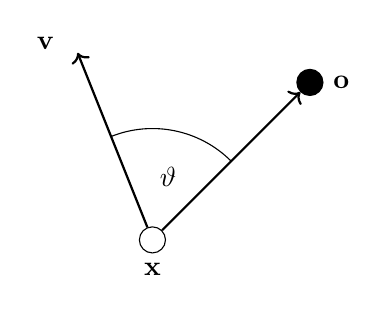
\begin{tikzpicture}
        	\node [label=below:{$\mathbf{x}$}, circle, draw=black] (human) at (0,0) {};
        	\node [label=right:{$\mathbf{o}$}, circle, draw=black, fill = black] (obstacle) at (2,2) {};
        	\node [label=left:{$\mathbf{v}$}] (vel) at (-1,2.5) {};
        	\draw [->, thick] (human) -- (vel);
        	\draw [->, thick] (human) -- (obstacle);
        	\draw (1,1) arc (45:112:1.4142);
        	\node () at (0.2,0.8) {$\vartheta$};
        \end{tikzpicture}
    \caption{Definition of the steering angle $\vartheta$.}
    \label{fig:steering_angle}
\end{figure}

We can now combine equation \eqref{eq:steering_angle_diff_eq} with the DMPs \cite{HPPS09}. The change in steering direction changes the velocity vector $\mathbf{v}$ as follows:
\[ \dot{\mathbf{v}} = \mathbf{R} \mathbf{v} \dot\vartheta, \]
where $\mathbf{R}$ is the rotational matrix with axis $\mathbf{r} = (\mathbf{o} - \mathbf{x}) \times \mathbf{v}$ and angle of rotation $\tfrac{\pi}{2}$, where $\mathbf{o}$ is the position of the obstacle.

The obstacle-induced change in velocity is embed in the motion equation by choosing
\begin{equation}
    \mathbf{p}(\mathbf{x},\mathbf{v}) = \gamma \mathbf{R} \mathbf{v} \vartheta \exp (-\beta \vartheta)
    \label{eq:obst_avoid_steering_angle}
\end{equation}
with 
\[ \vartheta = \arccos \left( { \frac{ \left\langle  {\mathbf{o} - \mathbf{x}}, {\mathbf{v}}\right\rangle }{|\mathbf{o} - \mathbf{x}| \cdot |\mathbf{v}|} }  \right) . \]

\begin{prop}[Hoffmann et al. \cite{HPPS09}]\label{prop:obstacle_convergence}
    Equation \eqref{eq:new_dmps_vector_acc} with \eqref{eq:obst_avoid_steering_angle} converges to the goal position $ \mathbf{g} $.
\end{prop}
\begin{proof}
    Since $ s \to 0 $ as $ t\to \infty $, we need to study the convergence of the reduced equation
    \[ \dot{\mathbf{v}} = \mathbf{K} (\mathbf{g} - \mathbf{x}) - \mathbf{D} \mathbf{v} + \gamma \mathbf{R} \mathbf{v} \vartheta \exp ( -\beta \vartheta ), \]
    where we set $ \tau = 1 $ for simplicity.\\
    Let us consider the Lyapunov function candidate $ V(\mathbf{x}, \mathbf{v}) $ defined as the energy of the linear spring system (with unit mass) $ \dot{\mathbf{v}} = \mathbf{K} ( \mathbf{g} - \mathbf{x} ) - \mathbf{D} \mathbf{v} $:
    \[ V(\mathbf{x}, \mathbf{v}) = \frac{1}{2} ( \mathbf{g} - \mathbf{x} )^\intercal \mathbf{K} ( \mathbf{g} - \mathbf{x} ) + \frac{1}{2} \mathbf{v}^\intercal \mathbf{v} . \]
    To prove convergence we have to prove that $ \dot{V} < 0 $ for $ \mathbf{v} \neq 0 $.
    Let us compute
    \begin{align*}
        \dot{V} (\mathbf{x}, \mathbf{v})
            & = \left\langle {\nabla_\mathbf{x} V(\mathbf{x}, \mathbf{v}))} , {  \dot{\mathbf{x}}} \right\rangle  + \left\langle {\nabla_\mathbf{v} V(\mathbf{x}, \mathbf{v}))} , {  \dot{\mathbf{v}}} \right\rangle  \\
            & = - ( \mathbf{g} - \mathbf{x} )^\intercal \mathbf{K} \mathbf{v} + \mathbf{v}^\intercal \dot{\mathbf{v}} \\
            & = - \mathbf{v} ^\intercal \mathbf{K} ( \mathbf{g} - \mathbf{x} ) + \mathbf{v} ^\intercal \mathbf{K} ( \mathbf{g} - \mathbf{x} ) - \mathbf{v} ^\intercal \mathbf{D}\mathbf{v} + \gamma \mathbf{v}^\intercal \mathbf{R} \mathbf{v} \vartheta \exp ( -\beta \vartheta ) \\
            & = -\mathbf{v} ^\intercal \mathbf{D} \mathbf{v} < 0.
    \end{align*}
    The damping matrix $ \mathbf{D} $ is positive definite by construction.
    The term $ \mathbf{v}^\intercal \mathbf{R} \mathbf{v} $ is zero since the matrix $\mathbf{R}$ is a rotation by 90 degrees.
    If $ \mathbf{v} = \mathbf{0} $ and $ \mathbf{x} \neq \mathbf{g} $, then $ \dot{V} = 0 $.
    However, if $ \mathbf{x} \neq \mathbf{g} $ then $ \mathbf{v} \neq \mathbf{0} $ and $V$ changes.
    Thus, according to LaSalle's theorem, $ \mathbf{x} $ converges to $ \mathbf{g} $.
\end{proof}

In the case of moving obstacles, we need to consider the relative velocity between the end-effector $\mathbf{x}$ and the obstacle $\mathbf{o}$, and not only the end-effector velocity $\mathbf{v}$ itself.
Therefore, we compute $\vartheta$ in the reference frame of the obstacle obtaining
\[ \vartheta = \arccos \left( { \frac{ \left\langle {\mathbf{o} - \mathbf{x}} , {\mathbf{v} - \dot{\mathbf{o}}} \right\rangle  }{|{\mathbf{o} - \mathbf{x}}| \cdot |{ \mathbf{v} - \dot{\mathbf{o}} } | } }  \right) , \]
where $\dot{\mathbf{o}}$ is the velocity of the obstacle.
The additional forcing term $\mathbf{p}(\mathbf{x},\mathbf{v})$ is defined as
\[ \mathbf{p}(\mathbf{x},\mathbf{v}) = \gamma \mathbf{R} ( \mathbf{v} - \dot{\mathbf{o}}) \vartheta \exp (-\beta \vartheta). \]
We remark that the proof of Proposition~\ref{prop:obstacle_convergence} does not hold for this perturbation term.

We remark that when more than one obstacles are present in the scene, it is sufficient to formulate $ \mathbf{p} (\mathbf{x}, \mathbf{v}) $ as the sum of the contributions of each obstacle.
Moreover, proof of Proposition~\ref{prop:obstacle_convergence} holds true even with multiple obstacles modeled as \eqref{eq:obst_avoid_steering_angle}.

\subsection{Volume Obstacles}

The methods described above can deal with point obstacles.
When dealing with real robotic situations, these methods may become numerically demanding since a dense point cloud may be necessary, and a different perturbation term $ \mathbf{p} $ has to be computed for each point, increasing the computational time.

For this reason, in \cite{GMCDSF19} and \cite{GMRSF20}, new methods to deal with obstacles with volume were developed.

The idea behind both methods lies in the definition of an \emph{isopotential} $C$ that describe the obstacles.
This isopotential is a function
\( C: \mathbb{R}^d \to \mathbb{R} \)
that vanishes on the boundary of the obstacle and increases as the distance from the obstacle boudary increases.
An example of isopotential is the following, which model an ellipse-shaped obstacle:
\[ C( \mathbf{x} ) = \left( \frac{x_1 - \hat{x}_1}{\ell_1} \right) ^ 2 + \left( \frac{x_2 - \hat{x}_2}{\ell_2} \right) ^ 2 - 1 , \]
where the ellipse is centered in $(\hat{x}_1, \hat{x}_2)$ and has semi-axis $\ell_1$ and $\ell_2$.
In \cite{GMCDSF19}, a static potential was proposed:
\[ U_S ( \mathbf{x} ) = \frac{A\,\exp(-\eta \,C( \mathbf{x} )}{C ( \mathbf{x} ) } . \]
In \cite{GMRSF20} a dynamic potential was proposed:
\[
    U_D( \mathbf{x} , \mathbf{v} ) =
    \begin{cases}
        \lambda (- \cos \theta) ^ \beta \, \frac{ \left\Vert \mathbf{v} \right\Vert  }{ C^\eta ( \mathbf{x} ) }
            & \text{if } \theta \in \left( \frac{\pi}{2}, \pi \right] \\ 
        0
            & \text{if } \theta \in \left[ 0 , \frac{\pi}{2} \right] 
    \end{cases}
    , 
\]
where
\[
\cos \theta = \frac{ \left\langle \nabla_ \mathbf{x} C( \mathbf{x} ) , \mathbf{v} \right\rangle  }{ \left\Vert \nabla_ \mathbf{x} C ( \mathbf{x} ) \right\Vert \left\Vert \mathbf{v} \right\Vert }
.
\]
In both cases, the perturbation term is written as the negative gradient (w.r.t. the position $ \mathbf{x} $) of the potential:
\begin{align*}
    \mathbf{p} _ S ( \mathbf{x} ) & = - \nabla _ \mathbf{x} U_S ( \mathbf{x} ), &
    \mathbf{p} _ D ( \mathbf{x}, \mathbf{v} ) & = - \nabla _ \mathbf{x} U_D ( \mathbf{x}, \mathbf{v} ).
\end{align*}

An example of all these methods can be seen in Figure~\ref{fig:obst_example}

\begin{figure}[t]
    \begin{subfigure}{0.3\linewidth}
        \includegraphics[width=\textwidth]{imgs/two_obst_point_static.png}
        \caption{Point static potential.}
    \end{subfigure}
    \hfill
    \begin{subfigure}{0.3\linewidth}
        \includegraphics[width=\textwidth]{imgs/two_obst_point_dynamic.png}
        \caption{Point dynamic potential.}
    \end{subfigure}
    \hfill
    \begin{subfigure}{0.3\linewidth}
        \includegraphics[width=\textwidth]{imgs/two_obst_point_steering.png}
        \caption{Steering angle method.}
    \end{subfigure}
    \\
    \begin{subfigure}{0.45\linewidth}
        \includegraphics[width=\textwidth]{imgs/two_obst_volume_static.png}
        \caption{Volume static potential.}
    \end{subfigure}
    \hfill
    \begin{subfigure}{0.45\linewidth}
        \includegraphics[width=\textwidth]{imgs/two_obst_volume_dynamic.png}
        \caption{Volume dynamic potential.}
    \end{subfigure}
    \caption{Examples of obstacle avoidance for DMPs.}
    \label{fig:obst_example}
\end{figure}

%%%%%%%%%%%%%%
%%  BIBLIO  %%
%%%%%%%%%%%%%%
\bibliographystyle{abbrv}
\bibliography{/home/michele/Documents/BIBLIO/biblio.bib}

\end{document}
